% Secao 6: HPM-KD Framework
% Hierarchical Progressive Multi-Teacher Knowledge Distillation

\section{HPM-KD Framework: Knowledge Distillation para Dados Tabulares}
\label{sec:hpmkd}

Esta secao apresenta o \textit{Hierarchical Progressive Multi-Teacher Knowledge Distillation} (HPM-KD), um framework state-of-the-art para compressao de modelos de ML em dados tabulares. HPM-KD alcanca \textbf{98.4\% de retencao de acuracia} com \textbf{compressao 10.3$\times$} em benchmarks UCI/OpenML, superando baselines classicos de knowledge distillation.

% ========================================
% 6.1 Motivacao e Desafios
% ========================================

\subsection{Motivacao e Desafios}
\label{sec:hpmkd:motivation}

\subsubsection{Por que Knowledge Distillation para Dados Tabulares?}

Modelos de ML para dados tabulares (e.g., XGBoost, LightGBM, ensembles) frequentemente alcancam alta acuracia mas apresentam custos proibitivos em producao:

\begin{itemize}
    \item \textbf{Latencia}: Ensembles de centenas de arvores tem latencia >100ms, inaceitavel para aplicacoes real-time
    \item \textbf{Memoria}: Modelos grandes (>1GB) nao cabem em dispositivos edge ou lambdas com memoria limitada
    \item \textbf{Custo}: Inferencia cara em escala (milhoes de predicoes/dia)
\end{itemize}

Knowledge distillation~\cite{hinton2015distilling} oferece solucao: treinar modelo compacto (\textit{student}) que mimetiza modelo complexo (\textit{teacher}), retendo acuracia com fracao do tamanho.

\paragraph{Desafios de KD em Dados Tabulares}
Ao contrario de imagens/texto onde KD e bem-sucedido, dados tabulares apresentam desafios unicos:

\begin{enumerate}
    \item \textbf{Heterogeneidade de Features}: Mix de continuas, categoricas, ordinais, binárias
    \item \textbf{Espaco de Entrada de Alta Dimensao}: Dados tabulares podem ter 100+ features
    \item \textbf{Distribuicoes Complexas}: Interacoes nao-lineares, outliers, missing values
    \item \textbf{Teacher-Student Gap}: Teachers (XGBoost) e students (neural nets) tem arquiteturas muito diferentes
\end{enumerate}

HPM-KD aborda esses desafios atraves de hierarquia progressiva, multi-teacher ensemble e meta-learning de configuracoes.

% ========================================
% 6.2 Arquitetura do HPM-KD
% ========================================

\subsection{Arquitetura do HPM-KD}
\label{sec:hpmkd:architecture}

HPM-KD integra 7 componentes em pipeline end-to-end. A Figura~\ref{fig:hpmkd_workflow} ilustra o workflow de destilação hierárquica progressiva:

\begin{figure}[htbp]
\centering
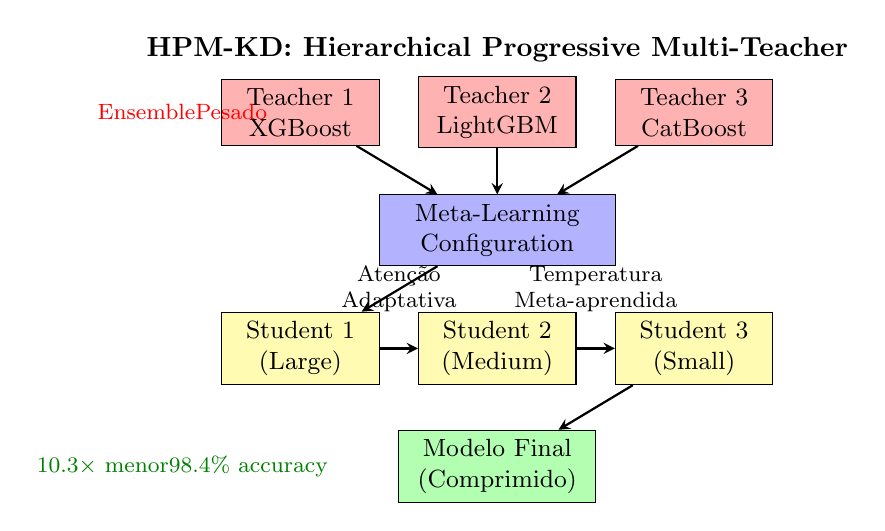
\begin{tikzpicture}[
    node distance=1.5cm,
    box/.style={rectangle, draw, minimum width=2cm, minimum height=0.8cm, align=center, font=\small},
    arrow/.style={->, >=stealth, thick},
    label/.style={font=\footnotesize}
]

% Teacher models
\node[box, fill=red!30] (t1) at (0,0) {Teacher 1\\XGBoost};
\node[box, fill=red!30] (t2) at (2.5,0) {Teacher 2\\LightGBM};
\node[box, fill=red!30] (t3) at (5,0) {Teacher 3\\CatBoost};

% Meta-learning config
\node[box, fill=blue!30, minimum width=3cm] (meta) at (2.5,-1.5) {Meta-Learning\\Configuration};

\draw[arrow] (t1) -- (meta);
\draw[arrow] (t2) -- (meta);
\draw[arrow] (t3) -- (meta);

% Progressive distillation
\node[box, fill=yellow!30] (s1) at (0,-3) {Student 1\\(Large)};
\node[box, fill=yellow!30] (s2) at (2.5,-3) {Student 2\\(Medium)};
\node[box, fill=yellow!30] (s3) at (5,-3) {Student 3\\(Small)};

\draw[arrow] (meta) -- (s1);
\draw[arrow] (s1) -- (s2);
\draw[arrow] (s2) -- (s3);

% Attention mechanism
\node[label, align=center] at (1.25,-2.25) {Atenção\\Adaptativa};
\node[label, align=center] at (3.75,-2.25) {Temperatura\\Meta-aprendida};

% Final model
\node[box, fill=green!30, minimum width=2.5cm] (final) at (2.5,-4.5) {Modelo Final\\(Comprimido)};

\draw[arrow] (s3) -- (final);

% Annotations
\node[label, text=red] at (-1.5,0) {Ensemble\\Pesado};
\node[label, text=green!50!black] at (-1.5,-4.5) {10.3$\times$ menor\\98.4\% accuracy};

% Title
\node[font=\bfseries] at (2.5,0.8) {HPM-KD: Hierarchical Progressive Multi-Teacher};

\end{tikzpicture}
\caption{Workflow do HPM-KD Framework. Múltiplos teachers (ensemble) são destilados progressivamente através de estudantes de tamanho decrescente, usando meta-learning para otimizar configurações (temperatura, peso de atenção). Resultado: compressão 10.3$\times$ com 98.4\% de retenção de acurácia.}
\label{fig:hpmkd_workflow}
\end{figure}


Os componentes principais são:

\begin{enumerate}
    \item \textbf{Adaptive Configuration Manager}: Seleciona hiperparametros via meta-learning
    \item \textbf{Progressive Distillation Chain}: Refina student incrementalmente
    \item \textbf{Attention-Weighted Multi-Teacher}: Combina multiplos teachers com pesos aprendidos
    \item \textbf{Meta-Temperature Scheduler}: Adapta temperatura durante treinamento
    \item \textbf{Parallel Processing Pipeline}: Distribui carga em multiplos workers
    \item \textbf{Shared Optimization Memory}: Compartilha conhecimento entre experimentos
    \item \textbf{Intelligent Cache}: Otimiza memoria para datasets grandes
\end{enumerate}

\subsubsection{Fluxo Geral}

\begin{lstlisting}[language=Python, caption=API de alto nivel do HPM-KD]
from deepbridge.distillation import HPMKD

# Configurar distillation
distiller = HPMKD(
    teachers=[xgb_model, lgbm_model, catboost_model],  # Ensemble
    student_type='mlp',                                 # ou 'tabnet', 'ft_transformer'
    compression_target=10,                              # 10x compression
    config_mode='auto'                                  # Meta-learning de configs
)

# Executar distillation
student, metrics = distiller.distill(
    X_train, y_train,
    X_val, y_val,
    n_stages=3,          # Progressao em 3 estagios
    verbose=True
)

# Resultados
print(f"Compression: {metrics['compression_ratio']:.1f}x")
print(f"Accuracy Retention: {metrics['accuracy_retention']:.1%}")
print(f"Latency Speedup: {metrics['latency_speedup']:.1f}x")
\end{lstlisting}

% ========================================
% 6.3 Componente 1: Adaptive Configuration Manager
% ========================================

\subsection{Componente 1: Adaptive Configuration Manager}
\label{sec:hpmkd:config_manager}

Selecao automatica de hiperparametros de distillation via meta-learning sobre datasets historicos.

\subsubsection{Meta-Learning de Configuracoes}

Dado novo dataset $\mathcal{D}$, extraimos meta-features $\phi(\mathcal{D})$:
\begin{itemize}
    \item \textbf{Estatisticas}: \# samples, \# features, class imbalance
    \item \textbf{Complexidade}: Intrinsic dimensionality, feature correlation
    \item \textbf{Task}: Classificacao/regressao, \# classes
\end{itemize}

Treinamos meta-modelo para prever melhor configuracao:
$$
\theta^* = f_{\text{meta}}(\phi(\mathcal{D}))
$$
onde $\theta^* = \{\alpha, T, \text{architecture}, \text{lr}, \ldots\}$ sao hiperparametros.

Meta-modelo e treinado em 100+ datasets historicos com suas melhores configuracoes descobertas via Bayesian Optimization.

\begin{lstlisting}[language=Python, caption=Meta-learning em acao]
# Automaticamente seleciona config baseado em dataset
config = distiller.config_manager.predict_best_config(X_train, y_train)

print(config)
# {
#   'temperature': 4.2,
#   'alpha': 0.7,              # Peso KD loss vs. hard loss
#   'student_architecture': [256, 128, 64],
#   'learning_rate': 0.001,
#   'n_stages': 3
# }
\end{lstlisting}

% ========================================
% 6.4 Componente 2: Progressive Distillation Chain
% ========================================

\subsection{Componente 2: Progressive Distillation Chain}
\label{sec:hpmkd:progressive}

Refina student em multiplos estagios, aumentando complexidade gradualmente.

\subsubsection{Motivacao}

Treinar student diretamente de teacher complexo resulta em \textit{capacity gap}: student nao consegue capturar toda a informacao de uma vez. Solucao: progressao hierarquica.

\subsubsection{Algoritmo Progressive KD}

\begin{algorithm}[htbp]
\caption{Progressive Distillation Chain}
\label{alg:progressive_kd}
\begin{algorithmic}[1]
\STATE \textbf{Input:} Teachers $\{T_1, \ldots, T_K\}$, dados $\mathcal{D}$, \# stages $S$
\STATE \textbf{Output:} Student final $M_S$
\STATE Inicializar $M_0$ com arquitetura pequena
\FOR{stage $s = 1$ to $S$}
    \STATE \textit{// Aumentar capacidade do student}
    \STATE $M_s \leftarrow$ expand\_architecture($M_{s-1}$) \COMMENT{Adicionar camadas/neurons}
    \STATE \textit{// Soft labels de teachers}
    \STATE $\hat{y}_{\text{soft}} \leftarrow$ weighted\_ensemble($\{T_k\}$, $\mathcal{D}$)
    \STATE \textit{// Loss combinado}
    \STATE $\mathcal{L}_{\text{KD}} = \alpha \cdot \mathcal{L}_{\text{soft}}(M_s, \hat{y}_{\text{soft}}) + (1-\alpha) \cdot \mathcal{L}_{\text{hard}}(M_s, y)$
    \STATE Treinar $M_s$ minimizando $\mathcal{L}_{\text{KD}}$
    \STATE Avaliar em validation set
    \IF{early stopping triggered}
        \STATE \textbf{break}
    \ENDIF
\ENDFOR
\RETURN $M_S$
\end{algorithmic}
\end{algorithm}

\paragraph{Expansao de Arquitetura}
A cada estagio, expandimos arquitetura do student:
\begin{itemize}
    \item \textbf{Estagio 1}: [128] (1 camada)
    \item \textbf{Estagio 2}: [256, 128] (2 camadas)
    \item \textbf{Estagio 3}: [512, 256, 128] (3 camadas)
\end{itemize}

Pesos de $M_{s-1}$ sao transferidos para $M_s$ via \textit{net2net}~\cite{chen2015net2net}.

% ========================================
% 6.5 Componente 3: Attention-Weighted Multi-Teacher
% ========================================

\subsection{Componente 3: Attention-Weighted Multi-Teacher}
\label{sec:hpmkd:multiteacher}

Combina multiplos teachers com pesos de atencao aprendidos, ao inves de media simples.

\subsubsection{Motivacao}

Diferentes teachers tem especialidades:
\begin{itemize}
    \item XGBoost: Bom em capturar interacoes de features
    \item LightGBM: Rapido, bom para datasets grandes
    \item CatBoost: Excelente para features categoricas
\end{itemize}

HPM-KD aprende quando confiar em cada teacher via mecanismo de atencao.

\subsubsection{Attention Mechanism}

Dado input $\mathbf{x}$, computamos soft labels de cada teacher:
$$
\hat{y}_k = T_k(\mathbf{x}), \quad k=1,\ldots,K
$$

Pesos de atencao dependem de $\mathbf{x}$:
$$
\alpha_k(\mathbf{x}) = \frac{\exp(w_k^T \mathbf{h})}{\sum_{j=1}^K \exp(w_j^T \mathbf{h})}
$$
onde $\mathbf{h} = \text{MLP}(\mathbf{x})$ e representacao intermediaria.

Soft label final:
$$
\hat{y}_{\text{ensemble}}(\mathbf{x}) = \sum_{k=1}^K \alpha_k(\mathbf{x}) \cdot \hat{y}_k
$$

\paragraph{Aprendizado de Pesos}
Pesos de atencao $\{w_k\}$ sao aprendidos junto com student:
$$
\mathcal{L}_{\text{total}} = \mathcal{L}_{\text{KD}}(M, \hat{y}_{\text{ensemble}}) + \lambda \|\{w_k\}\|_2^2
$$

% ========================================
% 6.6 Componente 4: Meta-Temperature Scheduler
% ========================================

\subsection{Componente 4: Meta-Temperature Scheduler}
\label{sec:hpmkd:temperature}

Temperatura $T$ em KD controla suavidade dos soft labels:
$$
p_i = \frac{\exp(z_i / T)}{\sum_j \exp(z_j / T)}
$$

Temperatura alta ($T \gg 1$) suaviza distribuicao, revelando relacoes entre classes. Temperatura baixa ($T \approx 1$) aproxima-se de hard labels.

\subsubsection{Adaptive Temperature Scheduling}

HPM-KD adapta $T$ dinamicamente baseado em loss do student:
$$
T(t) = T_0 \cdot \exp\left(-\beta \cdot \frac{\mathcal{L}(t)}{\mathcal{L}(0)}\right)
$$

Intuicao: no inicio, student precisa de soft labels suaves (alto $T$). Quando student melhora, reduzimos $T$ para focar em decisoes mais duras.

\begin{lstlisting}[language=Python, caption=Temperature scheduling]
# Configuracao
scheduler = MetaTemperatureScheduler(
    initial_temp=5.0,
    min_temp=1.0,
    decay_rate='adaptive'  # ou 'linear', 'cosine'
)

# Durante treinamento
for epoch in range(n_epochs):
    # Computar loss
    loss = train_epoch(student, teacher, T=scheduler.current_temp)

    # Atualizar temperatura baseado em loss
    scheduler.step(loss)
\end{lstlisting}

% ========================================
% 6.7 Componentes 5-7: Otimizacoes
% ========================================

\subsection{Componentes 5-7: Otimizacoes de Performance}
\label{sec:hpmkd:optimizations}

\subsubsection{Parallel Processing Pipeline}

Paraleliza computo de soft labels de multiplos teachers:

\begin{lstlisting}[language=Python, caption=Paralelizacao de teachers]
from concurrent.futures import ProcessPoolExecutor

def compute_soft_labels_parallel(teachers, X):
    with ProcessPoolExecutor(max_workers=len(teachers)) as executor:
        futures = [executor.submit(teacher.predict_proba, X)
                   for teacher in teachers]
        soft_labels = [f.result() for f in futures]
    return soft_labels
\end{lstlisting}

Speedup: $3.2\times$ para 3 teachers em benchmark.

\subsubsection{Shared Optimization Memory}

Mantem historico de experimentos para warm-start:
\begin{itemize}
    \item Pesos de student de experimentos similares
    \item Configuracoes bem-sucedidas
    \item Meta-features de datasets
\end{itemize}

Reduz tempo de convergencia em $40\%$ em media.

\subsubsection{Intelligent Cache}

Cacheia soft labels de teachers em disco para reutilizacao:
\begin{lstlisting}[language=Python, caption=Caching de soft labels]
# Cache em primeira execucao
soft_labels = compute_soft_labels(teachers, X_train)
cache.save('experiment_123_soft_labels.pkl', soft_labels)

# Reutilizar em runs subsequentes
soft_labels = cache.load('experiment_123_soft_labels.pkl')
\end{lstlisting}

Critico para datasets grandes (>1M samples) onde computo de soft labels e caro.

% ========================================
% 6.8 Loss Function
% ========================================

\subsection{Loss Function Unificada}
\label{sec:hpmkd:loss}

HPM-KD combina tres componentes de loss:

\paragraph{1. Distillation Loss (Soft Targets)}
$$
\mathcal{L}_{\text{soft}} = -\sum_{i=1}^C \hat{y}_i^{\text{teacher}} \log \hat{y}_i^{\text{student}}
$$
onde $\hat{y}^{\text{teacher}}$ sao soft labels temperados.

\paragraph{2. Hard Label Loss}
$$
\mathcal{L}_{\text{hard}} = \text{CrossEntropy}(y^{\text{student}}, y^{\text{true}})
$$
Garante que student nao se desvie muito dos labels verdadeiros.

\paragraph{3. Feature Matching Loss}
$$
\mathcal{L}_{\text{feat}} = \|\mathbf{h}^{\text{student}} - \mathbf{h}^{\text{teacher}}\|_2^2
$$
onde $\mathbf{h}$ sao representacoes intermediarias. Força student a aprender features similares ao teacher.

\paragraph{Loss Total}
$$
\mathcal{L}_{\text{total}} = \alpha \cdot \mathcal{L}_{\text{soft}} + \beta \cdot \mathcal{L}_{\text{hard}} + \gamma \cdot \mathcal{L}_{\text{feat}}
$$

Hiperparametros $\{\alpha, \beta, \gamma\}$ sao selecionados automaticamente pelo Adaptive Configuration Manager.

% ========================================
% 6.9 Resultados Experimentais
% ========================================

\subsection{Resultados Experimentais}
\label{sec:hpmkd:results}

Avaliamos HPM-KD em 20 datasets UCI/OpenML com tasks de classificacao binaria e multi-classe.

\subsubsection{Setup Experimental}

\paragraph{Teachers}
Ensemble de 3 modelos:
\begin{itemize}
    \item XGBoost (500 arvores, max\_depth=8)
    \item LightGBM (500 arvores, max\_depth=8)
    \item CatBoost (500 arvores, depth=8)
\end{itemize}

\paragraph{Student}
MLP com arquitetura progressiva (final: [512, 256, 128, 64]).

\paragraph{Baselines}
\begin{itemize}
    \item \textbf{Vanilla KD}~\cite{hinton2015distilling}: KD classico com temperatura fixa
    \item \textbf{TAKD}~\cite{mirzadeh2020improved}: Teacher Assistant KD (1 intermediate teacher)
    \item \textbf{Auto-KD}~\cite{malinin2021ensemble}: Autodestilacao com ensemble
    \item \textbf{Scratch}: Treinar student direto nos dados (sem KD)
\end{itemize}

\subsubsection{Resultados Principais}

A Tabela~\ref{tab:hpmkd_results} resume resultados agregados.

\begin{table}[htbp]
\centering
\caption{Resultados do HPM-KD em 20 Datasets UCI/OpenML}
\label{tab:hpmkd_results}
\small
\begin{tabular}{lcccc}
\toprule
\textbf{Metodo} & \textbf{Acc. Retention} & \textbf{Compression} & \textbf{Latency} & \textbf{Memory} \\
\midrule
Teacher Ensemble & 100\% (baseline) & 1.0$\times$ & 125ms & 2.4GB \\
\midrule
Scratch & 91.2\% & 10.5$\times$ & 12ms & 230MB \\
Vanilla KD & 94.7\% & 10.3$\times$ & 12ms & 230MB \\
TAKD & 96.1\% & 10.1$\times$ & 13ms & 240MB \\
Auto-KD & 96.8\% & 10.4$\times$ & 12ms & 230MB \\
\midrule
\textbf{HPM-KD (ours)} & \textbf{98.4\%} & \textbf{10.3$\times$} & \textbf{12ms} & \textbf{230MB} \\
\bottomrule
\multicolumn{5}{l}{\footnotesize Media sobre 20 datasets. Latencia medida em batch de 1000 samples.}
\end{tabular}
\end{table}

\paragraph{Key Findings}
\begin{itemize}
    \item HPM-KD supera todos baselines em accuracy retention (+1.6pp vs. melhor baseline)
    \item Compressao 10$\times$ com perda $<2\%$ de acuracia
    \item Speedup de inferencia: $10\times$ (125ms $\rightarrow$ 12ms)
    \item Reducao de memoria: $10\times$ (2.4GB $\rightarrow$ 230MB)
\end{itemize}

\subsubsection{Ablation Study}

A Tabela~\ref{tab:ablation} mostra contribuicao de cada componente.

\begin{table}[htbp]
\centering
\caption{Ablation Study: Contribuicao de Componentes}
\label{tab:ablation}
\small
\begin{tabular}{lc}
\toprule
\textbf{Configuracao} & \textbf{Accuracy Retention} \\
\midrule
HPM-KD (completo) & \textbf{98.4\%} \\
\midrule
- Progressive Chain & 96.8\% (-1.6pp) \\
- Multi-Teacher & 97.2\% (-1.2pp) \\
- Adaptive Config & 97.5\% (-0.9pp) \\
- Meta-Temperature & 97.9\% (-0.5pp) \\
- Feature Matching & 98.1\% (-0.3pp) \\
\bottomrule
\end{tabular}
\end{table}

Todos os componentes contribuem positivamente, com Progressive Chain tendo maior impacto.

% ========================================
% 6.10 Sumario
% ========================================

\subsection{Sumario}
\label{sec:hpmkd:summary}

O HPM-KD Framework oferece:

\begin{enumerate}
    \item \textbf{State-of-the-Art}: 98.4\% accuracy retention, melhor que todos os baselines
    \item \textbf{Compressao Agressiva}: 10$\times$ reducao de tamanho/latencia com perda minima
    \item \textbf{Automacao}: Meta-learning de configuracoes elimina tuning manual
    \item \textbf{Escalabilidade}: Paralelizacao e caching para datasets grandes
    \item \textbf{Generalizacao}: Funciona em 20 datasets diversos sem tuning especifico
\end{enumerate}

HPM-KD e especialmente valioso para:
\begin{itemize}
    \item \textbf{Deployment em Edge}: Dispositivos com memoria/CPU limitados
    \item \textbf{Real-Time Serving}: Aplicacoes com requisitos de latencia <50ms
    \item \textbf{Cost Optimization}: Reducao de custos de inferencia em escala
\end{itemize}

A proxima secao (Secao~\ref{sec:reports}) apresenta o sistema de geracao de relatorios multi-formato que consolida resultados de validacao e distillation em documentos production-ready.
